%%%%%%%%%%%%%
%  Frame 1  %
%%%%%%%%%%%%%
\begin{frame}
\frametitle{Stati stazionari}
\[
    r_i x_{i, s} \left(1-\sum_{j}^{n} a_{ij}x_{j, s}\right) = 0
\] 
\begin{itemize}
    \item $x_{i, s} = 0$, $i = 1, \ldots, n$.
    \item $\sum_{j}^{n} a_{ij}x_{j , s} = 1$, $i = 1, \ldots, n$.
    \item $x_{i, s} = 0$ con $i = 1, \ldots, k$ e $\sum_{j = 1}^{n} a_{lj}x_{j , s} = 1$ con $l = k+1, \ldots, n$.
\end{itemize}
\begin{center}
$2^n$ stati stazionari.
\end{center}
\end{frame}

%%%%%%%%%%%%%
%  Frame 2  %
%%%%%%%%%%%%%
\begin{frame}
\frametitle{Stati stazionari}
\framesubtitle{Esempi}
\begin{itemize}
    \item $n = 1$:
\[
    \frac{\text{d} x}{\text{d} t} = x(1-x) \implies  \begin{cases}
        x_{s,1} = 0 \quad \text{instab}\\
	x_{s, 2} = 1 \quad \text{stab}
    \end{cases}
\] 
\item $n=2$:
\[
\begin{dcases}
    \frac{\text{d} x}{\text{d} t} = r_0x(1-x - a_{12}y) = r_0x M_0(\v{x})  \\
    \frac{\text{d} y}{\text{d} t} = r_1y(1-a_{21}x - y) = r_1 y M_1(\v{x}) 
\end{dcases}
\quad \left[x_s, y_s\right] = 
\begin{cases}
    \left[0, 0\right] \quad \text{i}\\
    \left[0, 1\right] \quad \text{s}\\
    \left[1, 0\right] \quad \text{s}\\
    \left[\overline{x}, \overline{y}\right] \quad \downarrow
\end{cases}
\] 
\end{itemize}
\end{frame}

%%%%%%%%%%%%%
%  Frame 3  %
%%%%%%%%%%%%%
\begin{frame}
\frametitle{Stati stazionari}
\framesubtitle{Esempi: punto di coesistenza in 2D}
\[\begin{aligned}
    & \overline{x}= \frac{1-a_{12}}{1-a_{12}a_{21}} \\
    & \overline{y}= \frac{1-a_{21}}{1-a_{12}a_{21}}
\end{aligned}
\implies 
\begin{cases}
    a_{12} \text{ e } a_{21} > 1\\
    a_{12} \text{ e } a_{21} < 1
\end{cases}
\] 
\vspace{1em}
\[
J(\overline{x}, \overline{y}) =\begin{pmatrix}
    - r_0\overline{x} &  -r_0a_{12}\overline{x}\\ 
    -r_1a_{21}\overline{y} & - r_1\overline{y} \\
\end{pmatrix}
\]
\vspace{1em}
\[\begin{aligned}
    & T(J)  < 0\\
    & D(J) \propto 1 - a_{12}a_{21}
\end{aligned}
\implies 
\begin{cases}
    a_{12} \text{ e } a_{21} > 1 \implies  \text{ Sella}\\
    a_{12} \text{ e } a_{21} < 1 \implies  \text{ Pozzo}\\
\end{cases}
\]
\end{frame}

%%%%%%%%%%%%%
%  Frame 4  %
%%%%%%%%%%%%%
\begin{frame}
\frametitle{Carring Simplex}
\framesubtitle{Attracting set per il sistema}
\begin{equation}
    C_n \equiv  \left\{\v{x}\in \mathbb{R}^n_+ \ | \ \sum_{i}^{n} a_{ij} x_i = 1, \ i = 1, \ldots, n\right\}
    \label{eq:CS}
\end{equation}
\vspace{2em}
\[
    \text{dim}(C_n) = n-1
.\] 
\end{frame}

%%%%%%%%%%%%%
%  Frame 5  %
%%%%%%%%%%%%%
\begin{frame}
\frametitle{Carring Simplex}
\framesubtitle{Esempio in 3D}
\[
    C_3 = \left\{\v{x}\in \mathbb{R}^3_+ \ | \ \sum_{i}^{3} a_{ij}x_i = 1\right\} \qquad
    \text{dim}(C_3) = 2
.\] 
\begin{columns}
\begin{column}{0.4\textwidth}
    Su $C_3$ (piano di Figura \ref{fig:C3}) possono esistere (Poincare-Bendixon):
\vspace{1em}
\begin{itemize}
    \item Punti Fissi.
    \item Orbite Periodiche.
    \item Cicli Limite.
\end{itemize}
\end{column}
\begin{column}{0.4\textwidth}
\begin{figure}[h]
    \centering
    \captionsetup{width=.8\linewidth}
    \def\svgwidth{0.8\columnwidth}
    \input{figures/C3.pdf_tex}
    \caption{\scriptsize Punti dell'insieme $C_3$, la dinamica asintotica avviene su tale piano.}
    \label{fig:C3}
\end{figure}
\end{column}
\end{columns}
\end{frame}

%%%%%%%%%%%%%
%  Frame 6  %
%%%%%%%%%%%%%
\begin{frame}
\frametitle{Sistema in dimensione 4}
\[
    \frac{\text{d} x_i}{\text{d} t} = r_ix_i\left(1-\sum_{j}^{n} a_{ij}x_j\right)
\] 
\begin{center}
    Parametri in analisi:
\end{center}
\[
    r =\begin{bmatrix}
        1 \\
        0.72 \\
        1.53 \\
        1.27 \\
    \end{bmatrix} \qquad 
    a =\begin{bmatrix}
        1 & 1.09 & 1.52 & 0 \\
        0 & 1 & 0.44 & 1.36 \\
        2.33 & 0 & 1 & 0.47 \\
        1.21 & 0.51 & 0.35 & 1 \\
    \end{bmatrix}
\] 
\begin{center}
    Con questi il sistema esibisce un comportamento complesso (attrattore strano)
\end{center}
\end{frame}

%%%%%%%%%%%%%
%  Frame 7  %
%%%%%%%%%%%%%
\begin{frame}
\frametitle{Sistema in dimensione 4}
\framesubtitle{Stato stazionario di Coesistenza}
\begin{center}
Le soluzioni esplicite diventano complicate:
\end{center}
\[
    \overline{\v{x}} = \begin{pmatrix} \overline{x}_1 \\ 
                                       \overline{x}_2 \\ 
				       \overline{x}_3 \\ 
				       \overline{x}_4
		       \end{pmatrix} 
		       = \begin{pmatrix} 
			   0.3013 \\
			   0.4586 \\
			   0.1307 \\
			   0.3557
		       \end{pmatrix}
		       \quad  \text{es.:}  \quad \overline{x}_4 = \frac{NN}{DD}
\] 
\begin{tiny}
    \[\begin{aligned}
	DD =& a_{12} a_{21} a_{34} a_{43} - a_{12} a_{21} + 
	     a_{12} a_{23} a_{31} - a_{12} a_{23} a_{34} a_{41} + \\
	   & - a_{12} a_{24} a_{31} a_{43} + a_{12} a_{24} a_{41} +
	     a_{13} a_{21} a_{32} - a_{13} a_{21} a_{34} a_{42} + \\
	   & + a_{13} a_{24} a_{31} a_{42} - a_{13} a_{24} a_{32} a_{41}
	    - a_{13} a_{31} + a_{13} a_{34} a_{41} - a_{14} a_{21} a_{32} a_{43} +\\
	   & + a_{14} a_{21} a_{42} - a_{14} a_{23} a_{31} a_{42}  
	    + a_{14} a_{23} a_{32} a_{41} + a_{14} a_{31} a_{43} + \\
	   & - a_{14} a_{41} - a_{23} a_{32} + a_{23} a_{34} a_{42}
	    + a_{24} a_{32} a_{43} - a_{24} a_{42} - a_{34} a_{43} + 1\\
	   &\\
	NN =& a_{12} a_{21} a_{43} - a_{12} a_{21} + a_{12} a_{23} a_{31} + 
	      - a_{12} a_{23} a_{41} - a_{12} a_{31} a_{43} + a_{12} a_{41} + \\
	    & + a_{13} a_{21} a_{32} - a_{13} a_{21} a_{42} + a_{13} a_{31} a_{42} - a_{13} a_{31} - a_{13} a_{32} a_{41} + \\
	    & + a_{13} a_{41} - a_{21} a_{32} a_{43} + a_{21} a_{42} - a_{23} a_{31} a_{42} + a_{23} a_{32} a_{41} + \\
	    &  - a_{23} a_{32} + a_{23} a_{42} + a_{31} a_{43} + a_{32} a_{43} - a_{41} - a_{42} - a_{43} + 1
    .\end{aligned}\]
\end{tiny}
\end{frame}

%%%%%%%%%%%%%
%  Frame 8  %
%%%%%%%%%%%%%
\begin{frame}
\frametitle{Sistema in dimensione 4}
\framesubtitle{Analisi qualitativa degli stati stazionari}
\[
    J_{ij} = r_i \delta_{ij}\left(1-\sum_{j}^{4} a_{ij}x_j\right) - r_ix_ia_{ij}
.\] 
L'origine $Q_0$ è una sorgente mentre il punto di coesistenza $Q_{1234} \equiv \overline{\v{x}}$ è una sella:
\[
    J(\overline{\v{x}}) = \left.\frac{\text{d} x_i}{\text{d} x_j}\right|_{\overline{\v{x}}} = - a_{ij}r_i\overline{x}_i \implies 
	\begin{cases}
	    \lambda_{1,2}=0.0414 \pm i 0.1903\\
	    \lambda_3 = -0.3342 \\
	    \lambda_4 = -1.0319
	\end{cases}
\] 
\begin{center}
Ne restano altri 14\ldots
\end{center}
\end{frame}

%%%%%%%%%%%%%
%  Frame 9  %
%%%%%%%%%%%%%
\begin{frame}
\frametitle{Sistema in dimensione 4}
\framesubtitle{Analisi qualitativa degli stati stazionari}
\[
    J_{ij} = r_i \delta_{ij}\left(1-\sum_{j}^{4} a_{ij}x_j\right) - r_ix_ia_{ij}
.\]
\begin{itemize}
    \item $Q_i$ ($i = 1, \ldots, 4$): selle.
    \item $Q_{12}, Q_{14}, Q_{24}$ hanno $x_i < 0$.\\
	$Q_{13}, Q_{23}, Q_{34}$ selle.
    \item $Q_{124}$ sella. Unico con $x_i > 0$.
\end{itemize}
\end{frame}

%%%%%%%%%%%%%%
%  Frame 10  %
%%%%%%%%%%%%%%
\begin{frame}
\frametitle{Sistema in dimensione 4}
\framesubtitle{Analisi qualitativa degli stati stazionari}
\vspace{1em}
Gli stati $Q_1, Q_2, Q_3, Q_4, Q_{13}, Q_{23}, Q_{34}, Q_{124}$ giacciono su $C_4$.
\begin{figure}[H]
    \centering
    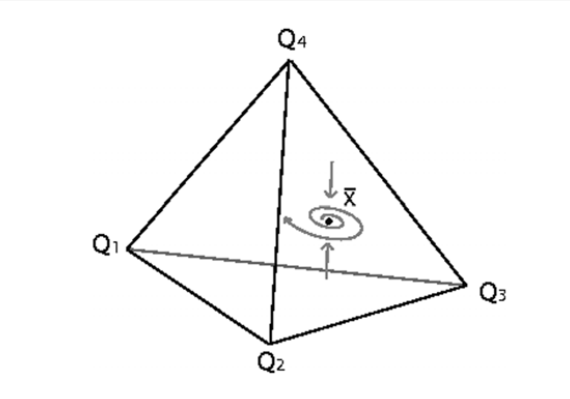
\includegraphics[width=0.35\textwidth]{figures/tetra.png}
    \def\svgwidth{0.45\columnwidth}
    \input{figures/tetra_open.pdf_tex}
    \caption{\scriptsize Tetraedro riportato da J. A. Vano et al in cui giacciono i punti stazionari (destra). Tetraedro aperto "revisionato" rispetto alla versione di J. A. Vano et al (sinistra).}
    \label{fig:figures-tetra_open-png}
\end{figure}
\end{frame}
